% vim:ts=4:sw=4
% Copyright (c) 2014 Casper Ti. Vector
% Public domain.
%!TEX root=../thesis.tex

\specialchap{序言}
% 中文测试文字。
现代的程序开发过程大量的依赖着对于API(Application Programming Interfaces,应用程序接口)的使用,因而在程序中进行API的替换也成为了程序开发过程以及软件维护过程中开发者的一项重要工作。其中,程序中的API改写主要可以分为以下两个类别。第一类是API的升级:当一个API推出的新版接口并不兼容旧版API接口时,使用旧版API的用户程序就需要进行改写来满足对于新API的使用。另一类则是API的切换,这一类情况常常出现在用户希望将原有的应用程序迁移到另一个平台上(例如从Android到IOS的程序切换),或是因为对于API性能以及维护功能上的其他需求而要求将原有的API切换到另一个API集合中去。在以上描述的这两种API更替场景中,我们需要将使用$API_1$的程序变换为使用$API_2$的程序,而$API_1$与$API_2$之间具有同构性,这样的替换也即相同功能之间的不同接口替换。然而,这样的程序变换并不容易。当用户手动进行这样的程序转换时,由于并非所有用户都是API的专家,他们并不能够全盘掌握两个API之间的映射关系,以及难以顾及到不同转换之间的交叉问题,手工的转换带来的结果就常常是错漏连篇的新程序,这带来结果就是更加高昂的软件维护成本和更多的人力资源消耗。

既然对于API升级的程序改写如此重要而又如此困难,让API发布者提供一个自动的程序转换工具就成为了帮助客户端程序员(即使用API的用户程序员)进行程序升级的一大利器:当API进行更新的时候,API发布者在发布API库的时候同时提供了一个用户升级工具来帮助客户进行程序升级,用户只需要让工具自动的将原有的程序进行改写就成为了使用新API的程序。让API提供者开发这样的转换工具具有相当的好处:一方面,作为API的专家,他具有更加丰富的API映射关系的知识,他能够处理还API之间的多方面映射关系,而另一方面,这样工具的开发是独立于用户程序的,一次开发就能够让广大用户都可以进行程序的升级,可以广泛的解决用户的需求问题。这样的工具例子有1)微软为了推广自己的.Net平台,提供了Visual Basic到Visual Basic.Net的程序转换工具,2)RIM提供了一个从Android到Blackberry的平台迁移工具,让使用Android API的程序能够自动改写为使用Blackberry的工具,从而可以让转换后的程序在Blackberry上运行而不需更多的工作。

然后,开发这样的Source-to-source自动转换工具并不容易。从转换工具的市场上来看,只有极小的一部分API拥有了这样的自动转换工具来完成程序的改写工作,其中一个重要的原因就是这些API间的程序自动转换工具常常会引入一些新的错误,或是在具体的程序环境中并不能完全按照API开发者的意图进行程序之间的改写。其中一个典型的例子就是Python 2to3.script工具,这个工具是设计来将使用python 2.x版本的程序升级为使用python 3.x版本的程序。虽然这个升级脚本能够在一定程度上完成对于python API的升级工作,但在升级过程中也引入了较多的错误,在有Pilgrim与Willison的案例研究\cite{python}中,2to3.script会导致包括类型错误在内的很多程序错误。从另一方面来看,程序变换开发的困难源自于专业开发环境的支持。由于并非所有的API开发者都能够熟悉程序语言的修改操作,让他们从底层开始实现这样的转换工具就显得困难重重。

事实上,为了解决程序变换的难题,程序语言社区设计出了很多的程序变换语言\cite{twinning}\cite{stratego}\cite{txl}。这些语言通过高层次的抽象来帮助使用者避开了底层开发中容易产生的错误,例如转换语言中能够保证程序变换前后不会产生语法错误,同时能够帮助开发者更好的描述自己需要表达的转换对象。然而对于API迁移这样一个特定场景的问题,这些变换语言的设计就显出了明显的不足,主要体现在以下几个方面:
\begin{itemize}
\item API变换过程中的类型安全并没有得到保证:这些通用的程序变换语言由于广泛的解决了多类的程序变换问题,类型安全就显得难以控制,而在较为单一的API升级问题中,变换对象保持在了statement以及expression层次上,类型的正确性就变得可控同时具有高层次的操作性。
\item API之间的映射没有得到高层次的抽象,因而这些转换仍然需要较多对于用户context的明确指定。由于API转换工具开发者需要能够在未知用户程序环境的情况下完成映射规则的指定,复杂的context就难以得到实现。
\item API升级之中多对多的API映射没有得到良好的支持:API之间的多对多问题涉及到了程序之间的环境分析问题以及转换语句之间的依赖关系问题,而大多数变换语言都是从语形上进行的转换,这样的转换就忽略了转换对象在运行时候的以来关系以及对应关系,从而导致了变换过程的实际语义遭到了违反。
\end{itemize}

我们接下来通过几个实际的例子来描述API之间程序改写中的常见问题。
\paragraph{类型安全问题} 类型安全问题主要体现在程序迁移前是类型正确的而改写之后出现了类型错误,举例如下。(该案例来自\cite{swing2swt})

在Java图形界面编程API Swing到SWT的升级过程中,Swing在创建一个窗口时需要首先创建一个Container来存放窗口中的内容,SWT也同理需要创建一个对应的Composite类来进行存放。(类图见\figref{swing2swtfig})因此在升级过程就就有了这样的两条对应关系(此处的规则只是简单的描述了API之间的映射关系,其中的$\pi_1$可以读作“将\code{Container}类的构造函数映射到\code{Composite}的构造函数,其中\code{Composite}的构造函数参数为\code{new Shell()}以及0”,第二条规则则是将\code{JList}类映射到\code{List}类,并将其构造函数进行对应的替换。):
\[
\begin{array}{ll}
	\pi_1=\code{new Container() ->> new Composite(new Shell(),0)}\\
	\pi_2=\code{new JList() ->> new List()}
\end{array}
\]
\begin{figure}[ht]
\centering
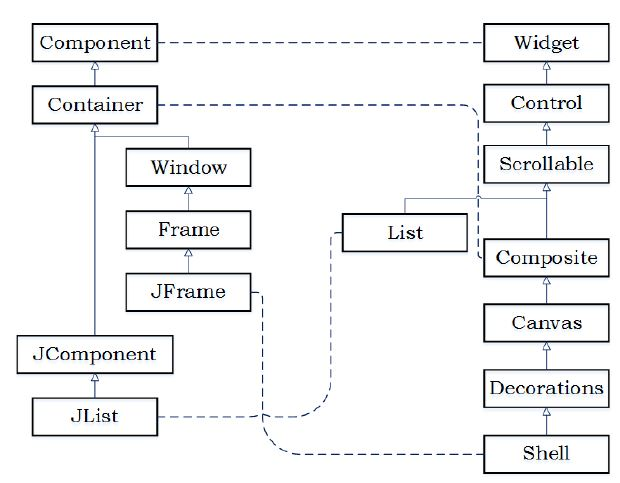
\includegraphics[width=200pt]{fig//swing2swt_class.JPG}
\caption{Swing(图左)到SWT(图右)之间的类图对应关系,其中虚线箭头表示两个API之间的类映射,实线箭头表示同一API中类的继承关系(往下为父类)}
\label{swing2swtfig}
\end{figure}
在这样的转换规则下,用于转换如下用户程序时就会出现类型的错误。
\[
\code{JList list = new Container();} \longrightarrow \code{List list = new Composite(new Shell(), 0);}
\]
其原因在于在\figref{swing2swtfig}中,Swing类型中的JList是Container的父类,因而左部满足子类关系而右部的List不再是Composite的子类,因而转换之前的类型是正确的,而转换之后就会导致类型错误的出现。

\paragraph{API之间多对多的映射问题}
比起前面所提到的类型问题,程序变换中更复杂的多对多问题更为引人注目。API之间多对多映射带来的主要问题则是用户程序上下文之间的不一致性,这样的问题并不像类型错误那样能够通过静态检查就能够得到并修复,而复杂的runtime错误让这类问题更容易隐藏。

在这里我们先简单使用程序匹配语言SmPL\cite{spatch}的语法来展示变换的规则。
\begin{center}
\begin{smpage}{0.25\columnwidth}
\begin{lstlisting}[style=patl]
(a:A->B) {
	- a.x();
	- a.y();
	+ a.z();
}
\end{lstlisting}
\end{smpage}
\end{center}
这一条规则就代表了一组API到另一组API之间的映射,元变量定义部分的\code{a:A->A}就代表了元变量在原来的API集合中类型为A,在新的API集合中类型为B,而这条规则表示了“每当遇到一个类型为A的变量a连续调用了a.x()与a.y()两个方法,我们就删除这两条语句,并用a.z()这样的一条语句来进行替换。”

假设我们现在的转换空间具有如下两条规则:
\begin{center}
\begin{smpage}{0.25\columnwidth}
\begin{lstlisting}[style=patl,frame=none]
(a:A->A) {
  - a.y();
  - a.x(); 
  + a.n(); 
}
\end{lstlisting}
~~~~{\small Rule-1}
\end{smpage}
\qquad\quad
\begin{smpage}{0.35\columnwidth}
\begin{lstlisting}[style=patl,frame=none]
(a:A->A,b:int->int) {
  - b = a.z();
  - a.x();
  + b = a.m(); 
}
\end{lstlisting}
~~~~{\small Rule-2}
\end{smpage}
\end{center}
让我们来考虑如下几种实际的转换类别来分析这两个例子的具体问题。
\begin{enumerate}
\item 情形1:在同一个context可以正确转换的例子。
\begin{center}
\begin{smpage}{0.3\columnwidth}
\begin{lstlisting}[style=patl,frame=none, numbers=none]
a.y();
a.x();
\end{lstlisting}
\end{smpage}
\begin{smpage}{0.6\columnwidth}
\begin{lstlisting}[style=patl,frame=none, numbers=none]
if (true) {
  a.y();
  a.x();
} else {
  b = a.z();
  a.x(); }
\end{lstlisting}
\end{smpage}
\end{center}
在这两个例子中,用户规则可以直接的在一个基本块中匹配到需要进行转换的语序序列,在类型和语形都能够正确匹配的情况下就能够进行正确的转换。因此可以比较容易的完成操作。
\item 情形2:被匹配的代码并不直接出现在连续块中,而需要进行调整来进行转换。
\begin{center}
\begin{smpage}{0.2\columnwidth}
\begin{lstlisting}[style=patl,frame=none, numbers=none]
b=a;
a.y();
b.x();
\end{lstlisting}
\end{smpage}
~
\begin{smpage}{0.2\columnwidth}
\begin{lstlisting}[style=patl,frame=none, numbers=none]
a.y();
i++;
a.x();
\end{lstlisting}
\end{smpage}
~
\begin{smpage}{0.48\columnwidth}
\begin{lstlisting}[style=patl,frame=none, numbers=none]
if (i<0) 
  a.y();
else 
  b = a.z();
a.x();
\end{lstlisting}
\end{smpage}
\end{center}
在上述的三个例子中,虽然并没有直接出现连续的转换指令,但是这些代码块却可以进行调整来使得代码变得可以转换。例如第一段代码中,由于\code{b}与\code{a}为alias关系,可以将\code{b.x();}重写为\code{a.x();},从而让转换可以正常进行。第二段代码中\code{i++;}与\code{a.x();}并没有依赖关系,从而可以交换位置让\code{a.y();a.x();}连续出现,因而也可以进行转换。第三段代码则可以通过将\code{a.x();}移动到两个分支语句中,从而让两个分支分别进行转换。
\item 情形3:类似于第二种情形,但是却因为以来关系的出现而无法转换。
\begin{center}
\begin{smpage}{0.44\columnwidth}
\begin{lstlisting}[style=java,frame=none, numbers=none]
b=a.z();
if (b<0) 
	a.x();
else
	a = new A();
\end{lstlisting}
\end{smpage}
\end{center}
在上面的这一段代码中,由于分支语句的条件\code{b<0}依赖于\code{b=a.z();},\code{b=a.z();}就不能像上述2-3的语句一样进行移动,从而产生了一个转换异常需要报告给用户。
\end{enumerate}

由于上述的种种困难,开发一个能够正确处理API之间程序改写的工具就显得尤为困难,因此在实际应用中,一个良好的程序转换工具应该能够保证独立于客户端程序的正确性:假设对于用户程序$p$,有一条在$p$上的性质$\phi$,那就需要对于一个转换程序$\Pi$,使得对于所有的$p$,都能够做到$\phi(p)$成立可以得出$\phi(\Pi(p))$也成立。这个关系可以形式化的表述为:
$$\forall p.\phi(p)\Longrightarrow\phi(\Pi(p))$$
在我们的目标中,我们就把性质$\phi$定义为类型正确性以及依赖关系的正确保持。
此外,让程序能够完全自动的转换任意的客户端程序而不会产生错误显然并不是一个可行的手段。实际进行程序变换的过程中,应当能够有规则检查系统来对转换程序进行检查,可以将规则的错误以及规则在非规范程序上可能产生的不正常表现报告给用户,从而让用户能够理解转换工具将在程序中进行的操作,并保证能够在所有错误正确处理的情况下就能够保证性质$\pi$的保持。这个关系可以由以下关系表示:

\begin{property}[Transformation Safety]
Given $p$,$\Pi$,if $\mathsf{check}(p,\Pi)==\code{true}$ and $\phi(p)$ holds, then $\phi(\Pi(p))$ holds, or else $\mathsf{check}(p,\Pi)$ will report warnings for the transformation.
\end{property}

除了对于转换目标正确性的支持,语言应当能够具有以下的特点以能够实际作为API之间程序变换问题的一个解决方案:
\begin{enumerate}
\item 能够高层次的描述API间的程序变换问题,表达能力要足够强,让用户能够表达绝大部分的API转换问题同时尽量减少对于非必要功能的依赖。
\item 转换规则的书写应当是独立于用户程序,需要能够保证作用在不同用户程序下都保持相同的转换特征。
\item 语言应当能够在用户程序中的API使用违反API使用规则时向用户提供错误信息,在转换前就能让用户知道需要进行修改的部分。
\end{enumerate}

本文主要就从语言机制的角度探讨了对于API之间程序改写问题的解决方案。本文设计了程序语言Patl,一种用具解决API升级问题中的多对多问题程序变换语言。本文的主要启示就在于将匹配放在了控制流图之中进行,并且在实际的程序改写之前进行一系列的语义等价转换,最后才在等价变换的程序变换基础上进行实际的API改写操作,同时在改写之中保持程序变化之间类型性质的转换正确性。

在接下来的章节中,我们首先会具体说明具体的研究问题难点,形式化的概述我们的解决方案(第一章),通过几个具体案例说明我们的解决方案(第二章),形式化的描述语言的语形语义(第三、四、五章),最后分析语言的应用以及在几个数据集下的分析结果(第六章)。

